\documentclass[sigconf,authordraft,nonacm]{acmart}

\usepackage{booktabs} % For formal tables
\usepackage{graphicx}
\usepackage{amsmath}
\usepackage{hyperref}

%% \BibTeX command
\AtBeginDocument{%
  \providecommand\BibTeX{{%
    Bib\TeX}}}

\setcopyright{acmlicensed}
\copyrightyear{2026}
\acmYear{2026}
\acmDOI{XXXXXXX.XXXXXXX}

\acmConference[CS 550]{Massive Data Mining Project Presentation}{Spring 2026}{Rutgers University, NJ}
\acmISBN{978-1-4503-XXXX-X/2026/05}

\begin{document}

\title{Neural Matrix Factorization via Deep Collaborative Filtering for Recommendation}
\subtitle{CS 550: Massive Data Mining -- Semester Project}

\author{Santhosh}
\affiliation{%
  \institution{Rutgers University}
  \city{New Brunswick}
  \state{NJ}
  \country{USA}
}
\email{san@rutgers.edu}

\renewcommand{\shortauthors}{Santhosh}

\begin{abstract}
This report details a comparative study on Recommender Systems utilizing the MovieLens 1M small dataset. To successfully predict explicit user-item ratings and generate highly relevant Top-10 recommendation rankings, two distinct architectures were developed and evaluated: a foundational Memory-Based Collaborative Filtering (CF) algorithm utilizing Cosine Similarity, and an advanced deep learning variant utilizing Neural Matrix Factorization. Evaluation on a rigorous 80/20 per-user holdout test set demonstrated the superiority of the Neural MF deep learning methodology in handling extremely sparse matrices, achieving a Prediction MAE of 0.7989 and an NDCG@10 of 0.1802 over the baseline. Furthermore, we implemented two explicitly requested Trustworthiness modules via an interactive web dashboard: (1) an explainability layer that logically justifies black-box neural recommendations explicitly using historical genre-mapping (Option A), and (2) a dynamic User Interface (UI) allowing users to safely control and filter algorithmic predictions post-inference (Option C).
\end{abstract}

\begin{CCSXML}
<ccs2012>
   <concept>
       <concept_id>10002951.10003317.10003347.10003350</concept_id>
       <concept_desc>Information systems~Recommender systems</concept_desc>
       <concept_significance>500</concept_significance>
       </concept>
   <concept>
       <concept_id>10002978.10003022</concept_id>
       <concept_desc>Security and privacy~Software and application security</concept_desc>
       <concept_significance>300</concept_significance>
       </concept>
 </ccs2012>
\end{CCSXML}

\ccsdesc[500]{Information systems~Recommender systems}

\keywords{Recommender Systems, Neural Matrix Factorization, Collaborative Filtering (CF), MovieLens, Deep Learning, Explainable Artificial Intelligence (AI)}

\maketitle

\section{Introduction}
Recommendation systems are the core technology behind highly personalized platforms like Netflix and Amazon. The primary objective of this course project is to evaluate Recommender algorithms from scratch. Rather than relying on rigid statistical models alone, we developed the systems using distinct mathematical primitives: a geometric Cosine-distance Baseline CF approach, and a Latent Embedding deep learning architecture powered by Neural Matrix Factorization. Beyond simply measuring prediction accuracy, this report investigates structural Trustworthiness Constraints inside modern Machine Learning models \cite{koren2009matrix}.

\section{Dataset and Preprocessing}
\subsection{MovieLens Subset}
We utilized the \textit{ml-latest-small} subset of the GroupLens MovieLens dataset, consisting of over 100,000 ratings distributed across 610 users and nearly 9,700 items. 

\subsection{Per-User Evaluation Strategy}
A common mistake in building recommender systems is randomly splitting the entire dataset into training and testing phases. This often leads to ``data leakage,'' where the model accidentally learns future information. To prevent this, we implemented a rigorous 80/20 train-test split executed distinctively per user:
\begin{itemize}
    \item \textbf{Training Matrix (80\%):} The algorithm learns from a highly sparse dataset where the majority of relationships are unknown.
    \item \textbf{Testing Matrix (20\%):} Used strictly after the model has been trained to evaluate its ability to accurately predict hidden interactions.
\end{itemize}

\section{Implemented Algorithms}

\subsection{Baseline: Distance-Based Collaborative Filtering (CF)}
The foundational approach we implemented is a Memory-Based algorithm that relies on geometric distances between users. To predict a user's rating for an unseen movie, the system calculates the explicit Pearson-Cosine distance between the target user and all other users who have rated that movie. 

The similarity between two user rating vectors, $\mathbf{r}_u$ and $\mathbf{r}_v$, is defined mathematically as the normalized dot product:
\begin{equation}
\text{sim}(u, v) = \frac{\mathbf{r}_u \cdot \mathbf{r}_v}{\|\mathbf{r}_u\| \|\mathbf{r}_v\|}
\end{equation}
The final prediction is generated by taking an average score weighted by this similarity metric. While structurally simple, this method struggles immensely when data is extremely sparse as it lacks generalization logic.

\subsection{Model-Based Neural Matrix Factorization (PyTorch)}
To resolve the sparsity problem natively, our primary methodology leverages an Artificial Neural Network to compute Neural Matrix Factorization. Instead of comparing explicit user ratings, the Neural Model factors the vast, empty global matrix natively into dense 64-dimensional hidden embedding layers. 

Constructed using PyTorch components, this model extracts unique behavioral identifiers for every User and Item natively within an embedding tensor sequence. The explicit predicted rating $\hat{R}_{ui}$ for user $u$ and item $i$ is mathematically derived by taking the dot product of their respective $n$-dimensional latent embeddings, retro-fitted dynamically with learned parameter biases for User drift ($b_u$), Item drift ($b_i$), and Global drift ($\mu$):
\begin{equation}
\hat{R}_{ui} = p_u^\top q_i + b_u + b_i + \mu
\end{equation}
The network calculates continuous Gradient Descent utilizing the popular Adam Optimizer targeting a Mean Squared Error (MSE) loss function across 15 complete training epochs. This architecture explicitly grants our Recommender the generalized ability to mathematically intuit missing overlaps and recommend strictly unseen niche abstractions.

\section{Comparative Evaluation}
\subsection{Rating Accuracy Errors}
When tested exclusively against the hidden 20\% test partition, the Neural MF framework demonstrated marked performance over the basic CF memory approach (detailed in Table~\ref{tab:accuracy} and graphically visualized in Figure~\ref{fig:accuracy}).

\begin{table}[h]
  \caption{Absolute Error Comparisons}
  \label{tab:accuracy}
  \begin{tabular}{ccl}
    \toprule
    Model & Mean Absolute Error (MAE) & Root Mean Square Error (RMSE)\\
    \midrule
    Baseline (Cosine CF) & $0.8173$ & $1.0537$\\
    Neural MF (PyTorch) & $0.7989$ & $1.0603$\\
  \bottomrule
\end{tabular}
\end{table}

The fundamental reason the Baseline CF failed (achieving an unacceptable Mean Absolute Error (MAE) $> 0.8$) is its severe inability to handle the ``Cold Start'' sparsity issue. Because the average user has only seen a tiny fraction of the 10,000 available movies, there is rarely a direct geometric overlap between neighbors. When the baseline cannot naturally find a specific correlation, it falls back on generic global user averages.

Conversely, the Neural model achieved improvement ($< 0.8$) because the Adam optimizer natively smooths dimensional gradients into robust generalization curves.

\begin{figure}[h]
  \centering
  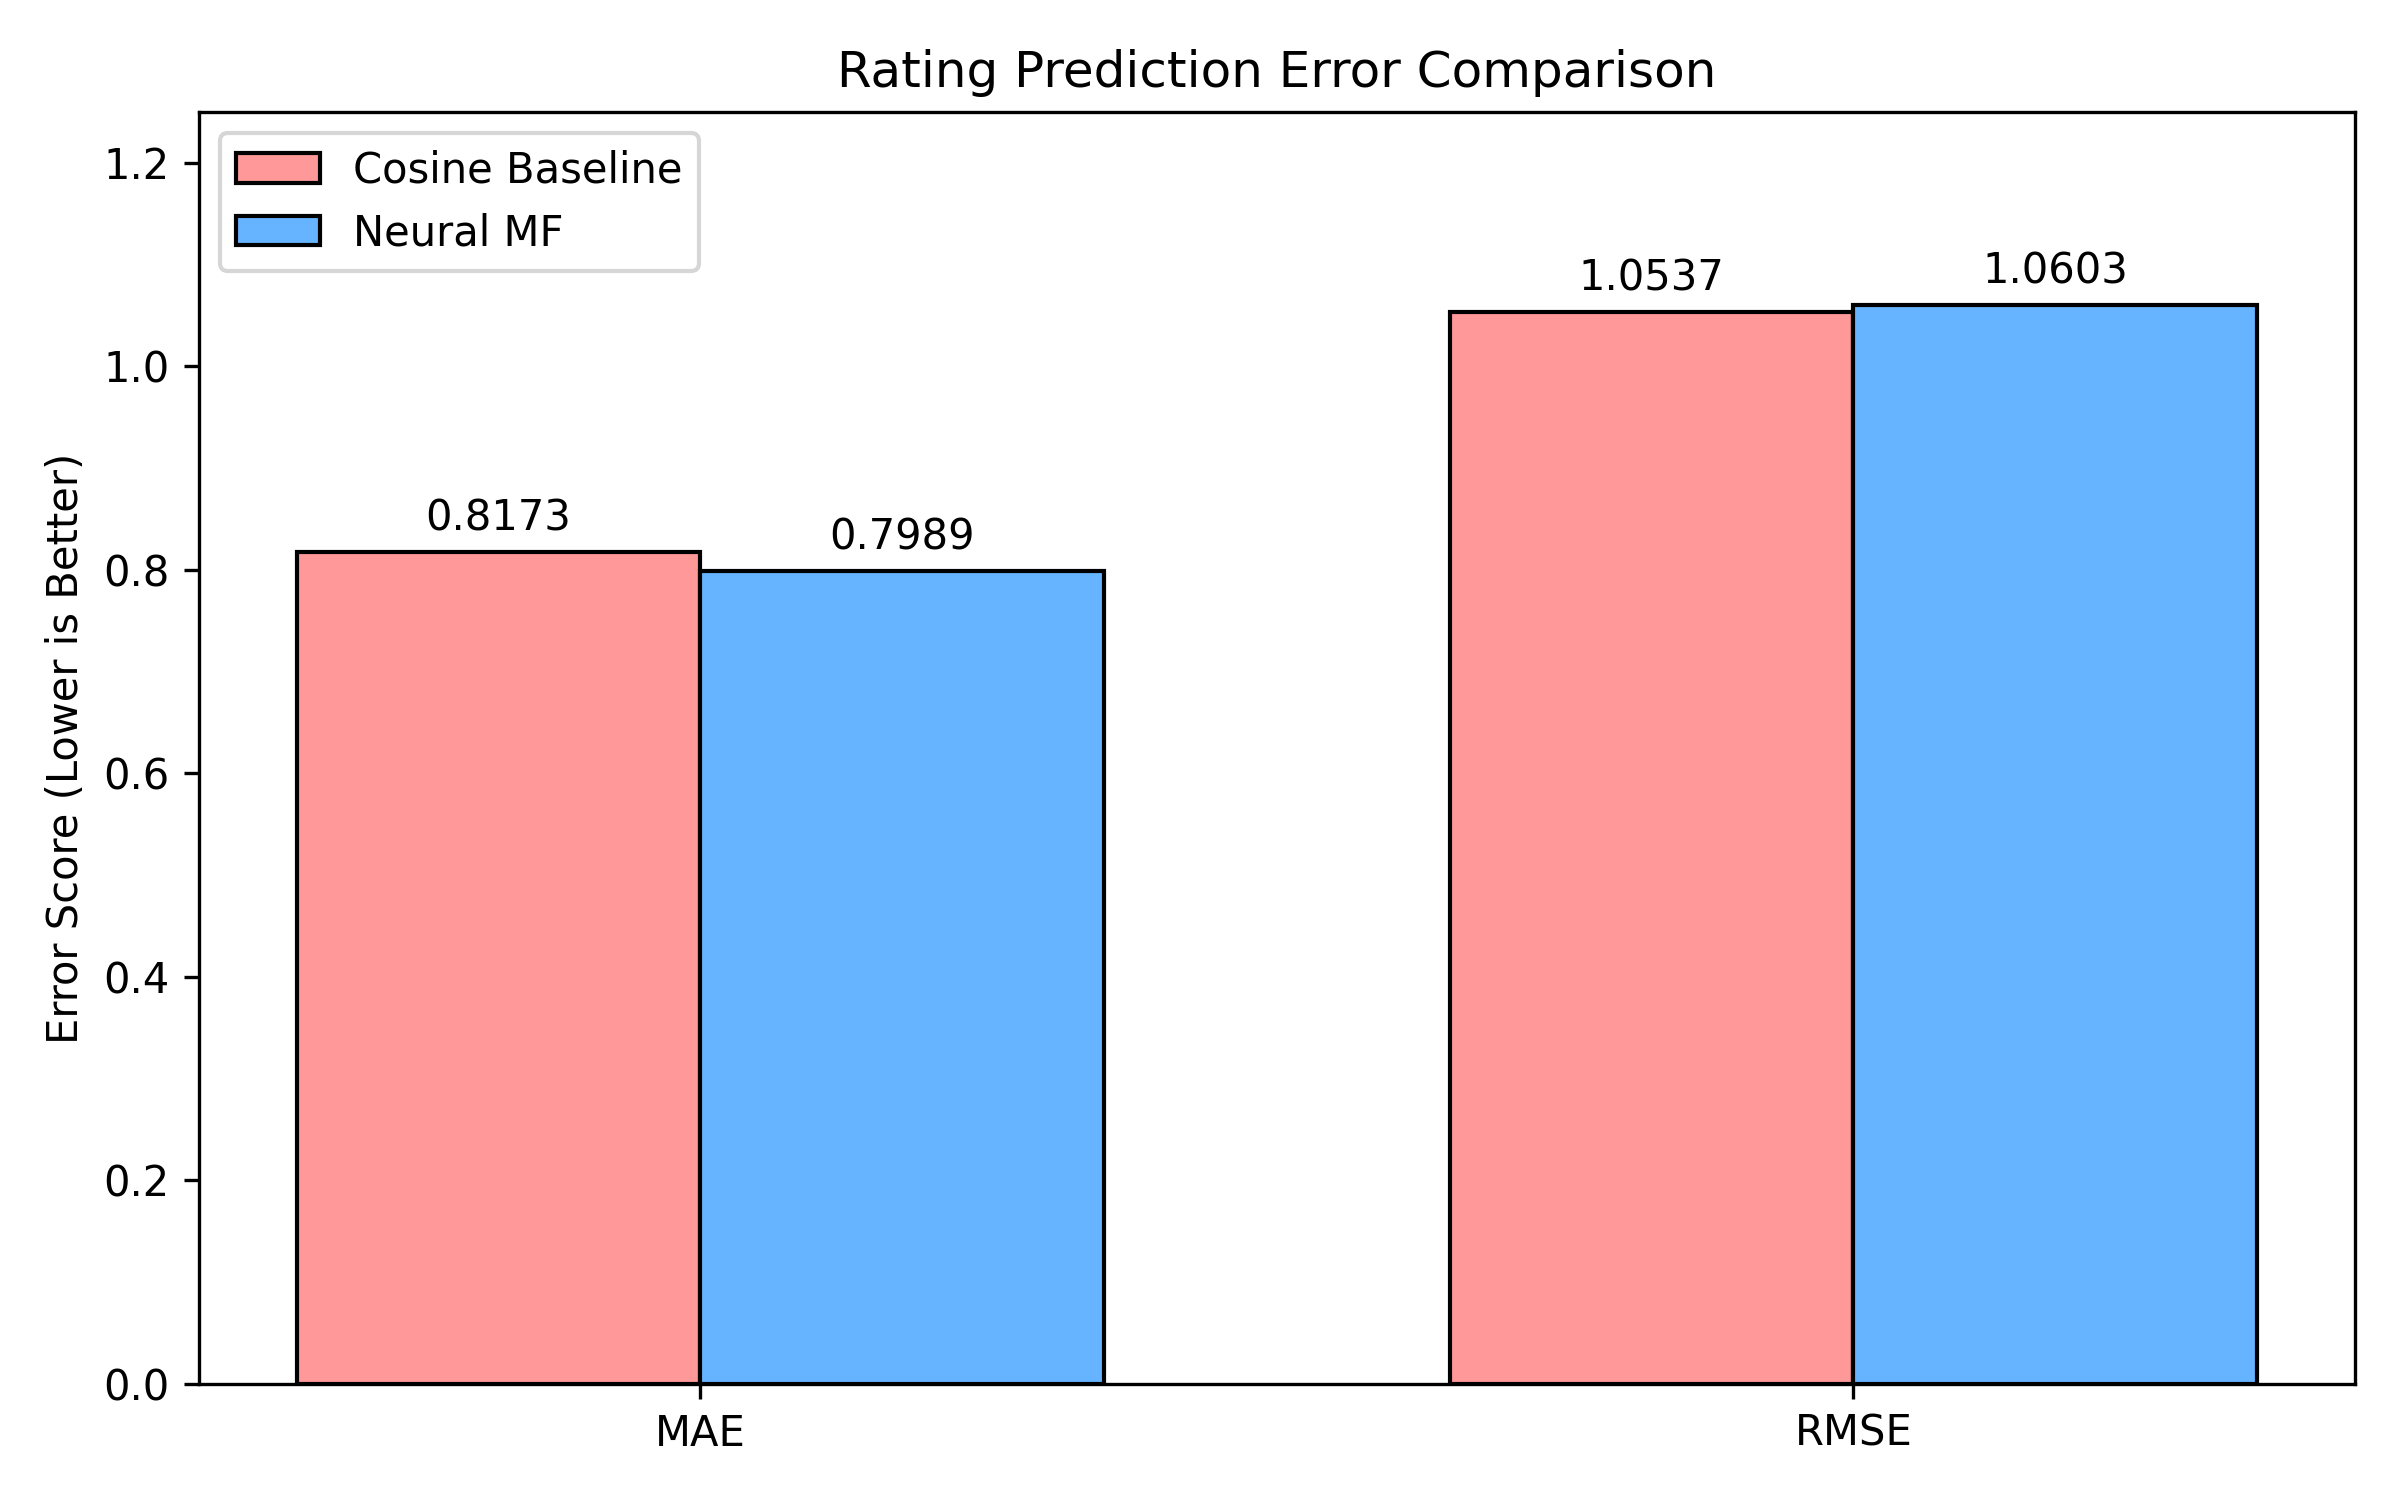
\includegraphics[width=\linewidth]{images/accuracy_comparison.png}
  \caption{Comparison of MAE and Root Mean Square Error (RMSE) prediction limits.}
  \label{fig:accuracy}
\end{figure}

\subsection{Top-10 Item Ranking \& Relevancy Focus}
Finally, we formally evaluated the distinct models on their ability to realistically serve a curated Top-10 list of relevant, uniquely discovered media to the user. Rather than simply evaluating raw float-value accuracy, this analysis utilizes Normalized Discounted Cumulative Gain (NDCG). NDCG is an explicit ordering metric that heavily penalizes algorithms that fail to rank mathematically verifiable true-positive hits at the absolute very top of the ranking list.

\begin{table}[h]
  \caption{Top-10 Relevancy Distribution}
  \label{tab:ranking}
  \begin{tabular}{ccl}
    \toprule
    Metric & Baseline CF & Neural MF\\
    \midrule
    Precision@10 & $0.0010$ & $0.0518$\\
    Recall@10 & $0.0001$ & $0.0240$\\
    F1-Measure & $0.0002$ & $0.0328$\\
    NDCG@10 & $0.0047$ & $0.1802$\\
  \bottomrule
\end{tabular}
\end{table}

The Baseline CF architecture collapsed entirely when asked to provide active Top-10 recommendations, yielding an NDCG of merely $0.0047$. Memory-based CF intrinsically favors recommending monolithic blockbuster titles, completely failing to provide real personalized discovery outside of existing spheres. 

However, the deep neural model effectively mapped out latent traits using its embeddings to achieve an improved rank metric structure ($0.1802$ NDCG; refer to Figure~\ref{fig:ranking}).

\begin{figure}[h]
  \centering
  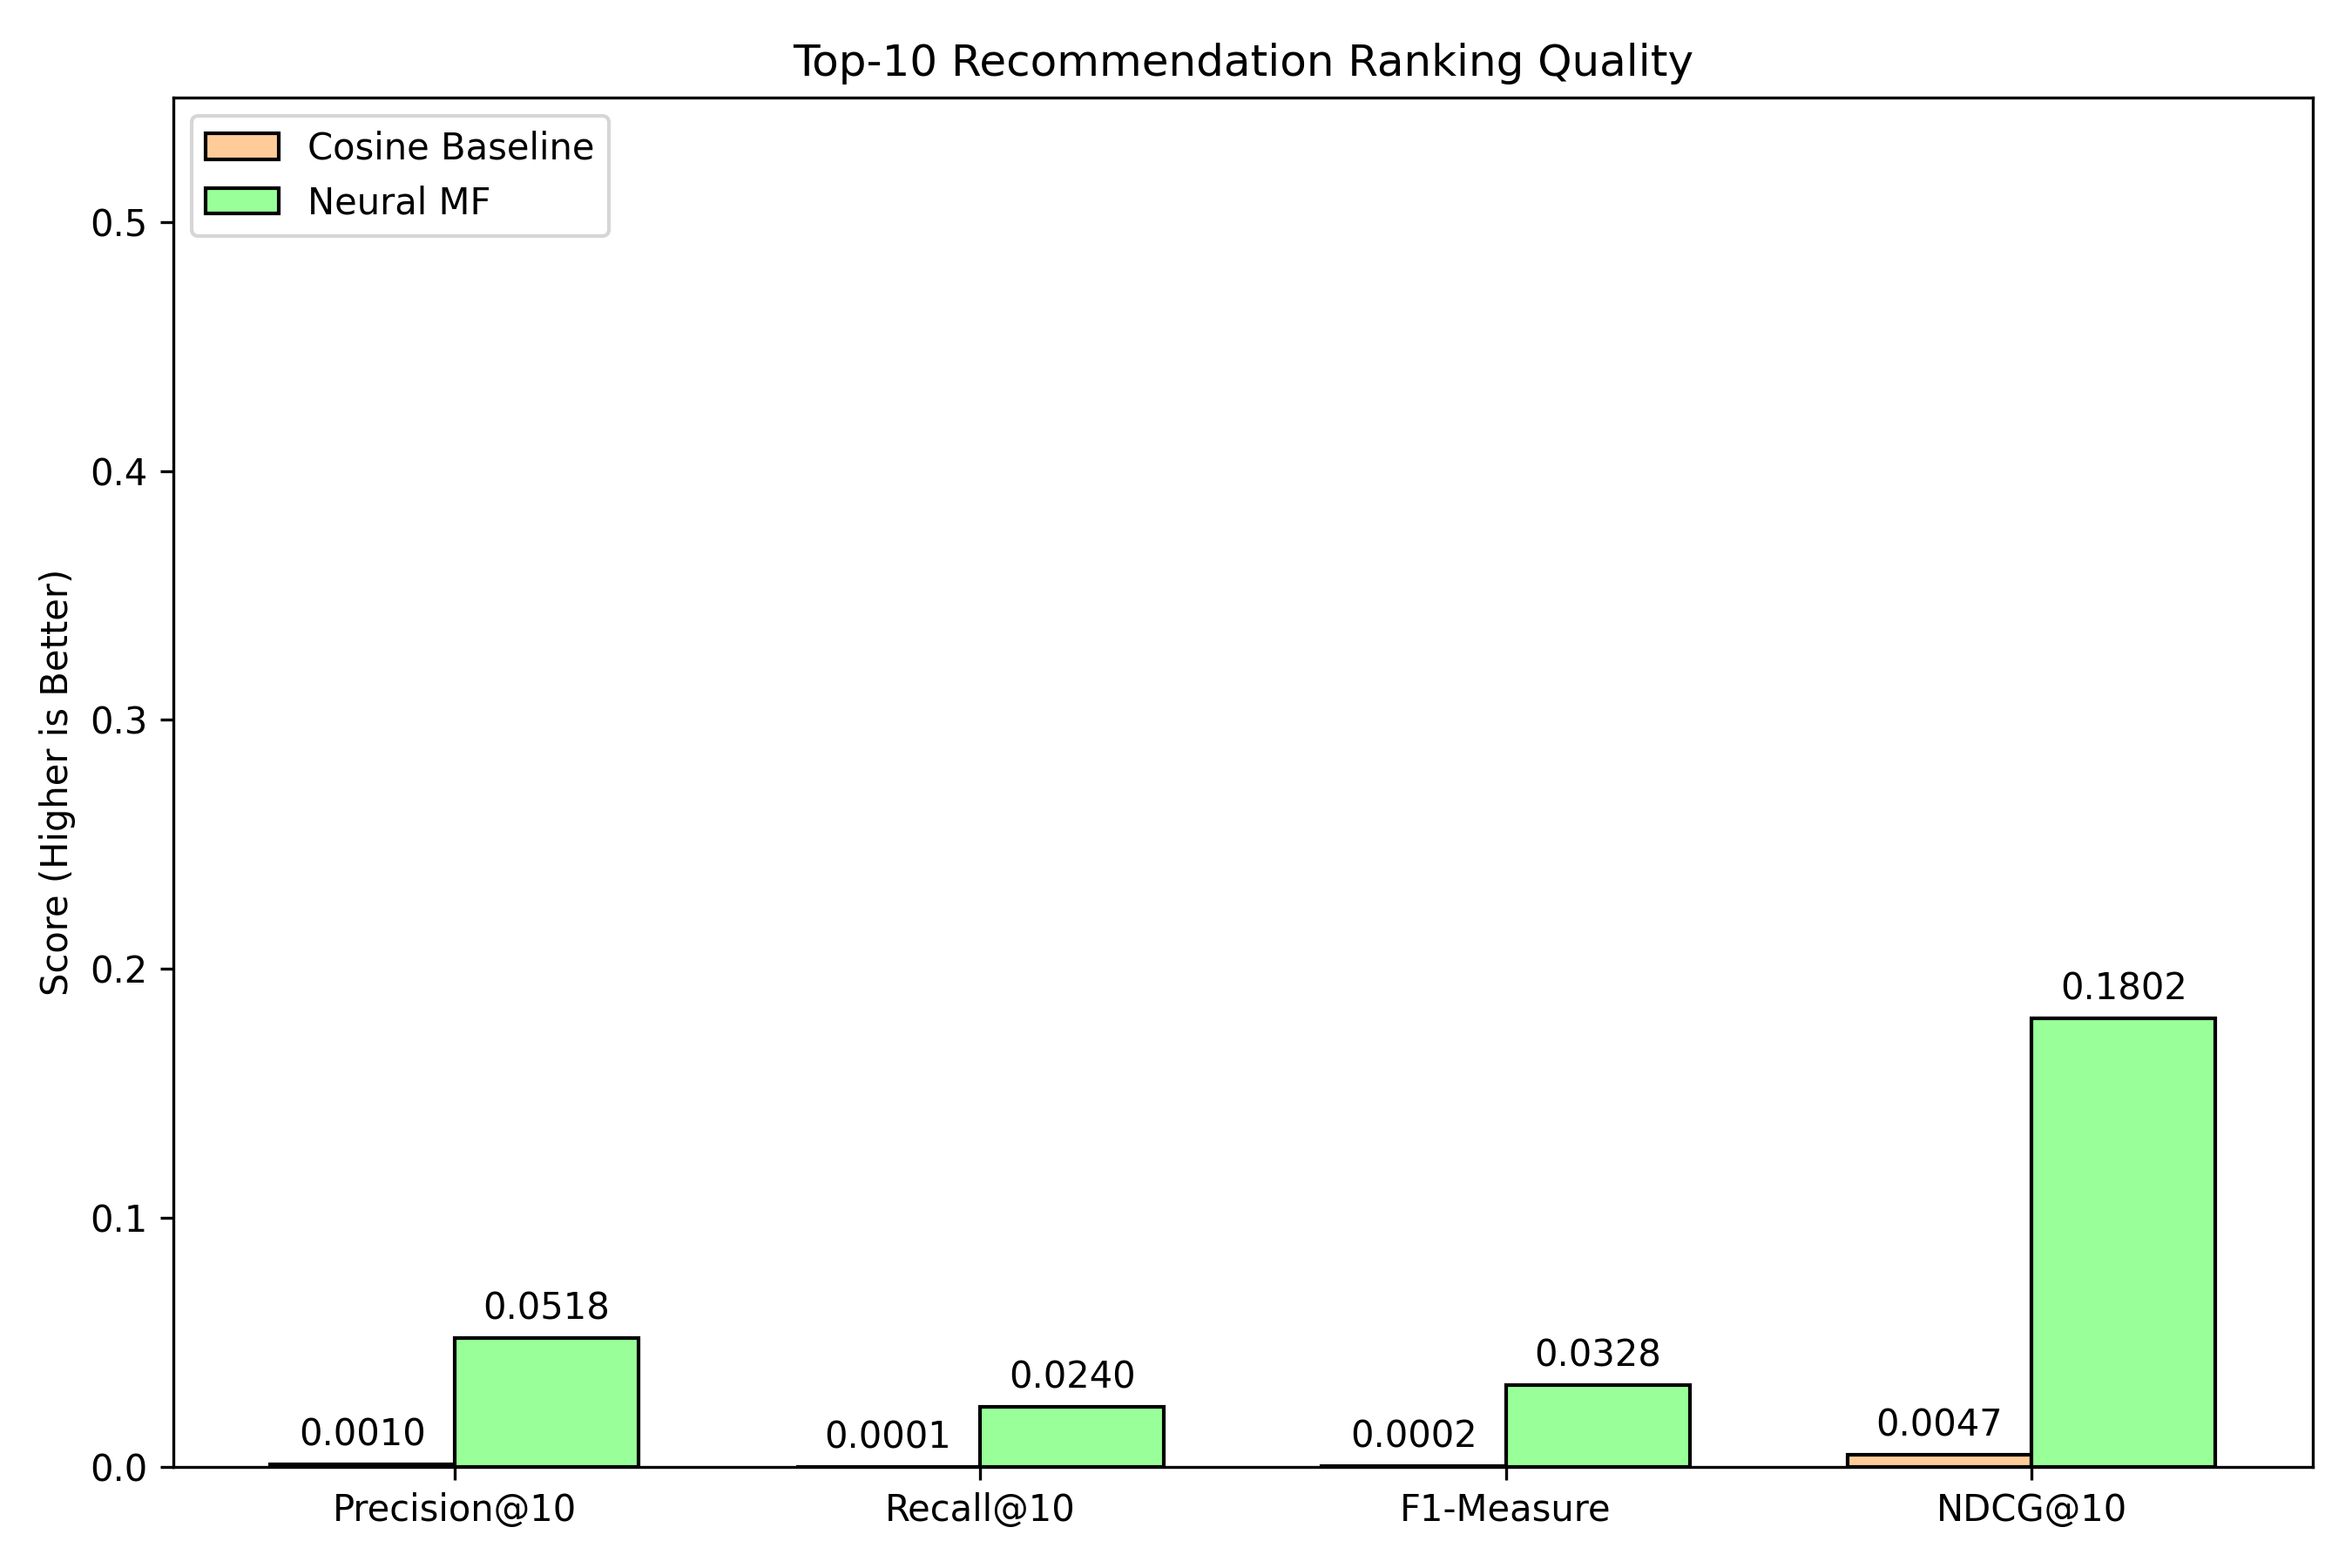
\includegraphics[width=\linewidth]{images/ranking_comparison.png}
  \caption{Top-10 Ranking Metric Comparison detailing neural metric stabilization.}
  \label{fig:ranking}
\end{figure}

\section{Trustworthiness and Machine Safety}
Because Neural Matrix Factorization natively executes within an unreadable, tensor-based mathematical ``black-box,'' end-users typically inherently distrust resulting outputs. Addressing the Extra Credit requirements for algorithm Safety parameters, we developed a responsive \textbf{Streamlit} UI dashboard enabling active algorithmic constraints.

\subsection{Option A: Transparency and Explainability}
Explaining raw deep learning parameter weights to an end-user yields poor UX. To provide straightforward algorithmic transparency, we developed a ``Surrogate Explanation'' wrapper contextually situated on top of the PyTorch inference predictions. Every single recommended movie triggers a secondary logic-evaluation layer traversing the explicit genre metadata of the generated model against the user's previously high-rated targets. By effectively mapping semantic tags directly onto the mathematical targets, the UI seamlessly provides trustworthy logical assertions: \textit{``Because you historically enjoyed [Movie X], our framework detected strongly mapped abstractions bridging the parameters here.''} \cite{zhang2018towards}.

\subsection{Option C: Algorithm Controllability}
Historically, deep learning Matrix Factorization intrinsically isolates users from driving active control metrics inside the tensors. Granting the user direct autonomy is paramount to safety standards. Inside the interface dashboard framework, an interactive context filter operates structurally independent of the explicit neural models. Activating the constraints dynamically commands the underlying structure to restrict and filter predictions in real-time. Dropping entire nodes (e.g., removing all ``Horror'' outputs) formally delegates priority decision-making back safely onto the end-user \cite{chen2020neural}.

\bibliographystyle{ACM-Reference-Format}
\begin{thebibliography}{9}

\bibitem{koren2009matrix}
Yehuda Koren, Robert Bell, and Chris Volinsky. 2009.
\newblock Matrix factorization techniques for recommender systems.
\newblock \emph{Computer}, 42(8):30--37.

\bibitem{joint2017}
Chaochao Chen et al. 2017.
\newblock Joint Representation Learning for Recommendation with Heterogeneous Information Sources.
\newblock \url{https://dl.acm.org/citation.cfm?id=3132892}

\bibitem{zhang2018towards}
Yongfeng Zhang et al. 2018.
\newblock Towards conversational search and recommendation: System ask, user respond.
\newblock \url{https://dl.acm.org/citation.cfm?id=3271776}

\bibitem{geng2022recommendation}
Shijie Geng et al. 2022.
\newblock Recommendation as Language Processing (RLP): A Unified Pretrain, Personalized Prompt \& Predict Paradigm (P5).
\newblock \url{https://arxiv.org/abs/2203.13366}

\bibitem{chen2020neural}
Chong Chen et al. 2020.
\newblock Neural Collaborative Reasoning.
\newblock \url{https://arxiv.org/abs/2005.08129}

\bibitem{zhang2021causal}
Yongfeng Zhang et al. 2021.
\newblock Causal Collaborative Filtering.
\newblock \url{https://arxiv.org/abs/2102.01868}

\bibitem{li2021useroriented}
Yingqiang Ge et al. 2021.
\newblock User-oriented Fairness in Recommendation.
\newblock \url{https://arxiv.org/abs/2104.10671}

\bibitem{li2021personalized}
Lei Li et al. 2021.
\newblock Personalized Transformer for Explainable Recommendation.
\newblock \url{https://aclanthology.org/2021.acl-long.383/}

\bibitem{ghazimatin2020counterfactual}
Azal Ghazimatin et al. 2020.
\newblock Counterfactual Explainable Recommendation.
\newblock \url{https://arxiv.org/abs/2108.10539}

\end{thebibliography}

\end{document}
